\chapter{Multi-Level Modeling and Metadepth}

This chapter continues where chapter 2 left off. Now that we know we can capture the important domain concepts and their relationships through the modeling language standard UML, we can address issues with the object-oriented paradigm currently underpinning the UML. UML supports modeling at two levels only, e.g. in the form of object diagrams (instance level) and class diagrams (type level). Thus, it provides only meager support for true multi-level modeling. As a consequence, this two-level modeling approach adds accidental complexity to domain models. A possible solution involves the use of \textit{powertypes}. Another solution introduces an object that can capture both \textit{classlike} and \textit{objectlike} features, \textit{clabjects}, together with the concept of potency to support an arbitrary number of modeling levels. Both concepts are explained in depth. Finally, Metadepth, a framework for multi-level meta-modeling is presented. This approach solves the mismatch between the two-level modeling paradigm and the information it models.

\section{Deep Meta-Modeling}

A question that undoubtedly comes to ones mind is the following: "Is it possible to keep the simplicity of figure ~\ref{fig:types_classes} while still supporting the ability to create new product types at runtime?". In order to make this possible, the type level should be as dynamic as the object level. We should of course have some control over what types can be created and what features they possess. Therefore, we need (domain-)meta-types controlling the features of (domain-) types \cite{AccidentalComplexity}. However, the problem with the "Item Description" pattern is that it uses three classification levels, where only two level (class/object) mechanisms are supported. This introduces a level mismatch problem, depicted in figure ~\ref{fig:mapping_inconsistent}. It shows that our example actually features \textit{three} ontological levels, while the corresponding models only contain \textit{two} modeling levels. The level of the model instance is used to represent two ontological levels, domain types and domain instances.
\begin{figure}[h!]
\centering
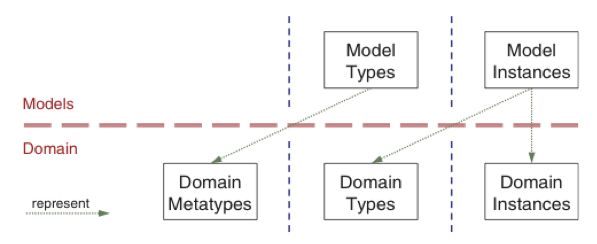
\includegraphics[width=0.9\textwidth]{images/chap3_mapping_inconsistent.png}
\caption{Mapping domain levels to modeling levels.}
\label{fig:mapping_inconsistent}
\end{figure} \\
In the following section, we will discuss how it is possible to avoid squeezing multiple domain levels in only two modeling levels.

\subsection{Clabject}

In order to truly support multiple levels, we need modeling concepts that can be applied in a uniform way across all levels in a multilevel hierarchy \cite{AccidentalComplexity}. A modeling construct that supports the representation of the dual �type and object�-property of some domain concept is necessary. Therefore, the concept of \textit{clabject} was introduced. Clabjects are a combination of \textit{class} and \textit{object}. They have a name and a set of attributes, like classes, and a set of slots, like objects. The example of the previous section, modeled using clabjects, is depicted in figure ~\ref{fig:model_clabject}. This solution features less accidental complexity than solutions of previous sections, because it maximizes the mapping between the problem structure and the solution structure. Note that the model types do not contain attributes, they only fill in slots, which are instantiations of attributes found in a \textit{higher} modeling level. In figure ~\ref{fig:model_clabject}, the model instances do not contain any slots, because all attributes are already instantiated as slots at the model types level. Furthermore, we have used only a single notion of the \textit{instance-of} relationship.
\begin{figure}[h!]
\centering
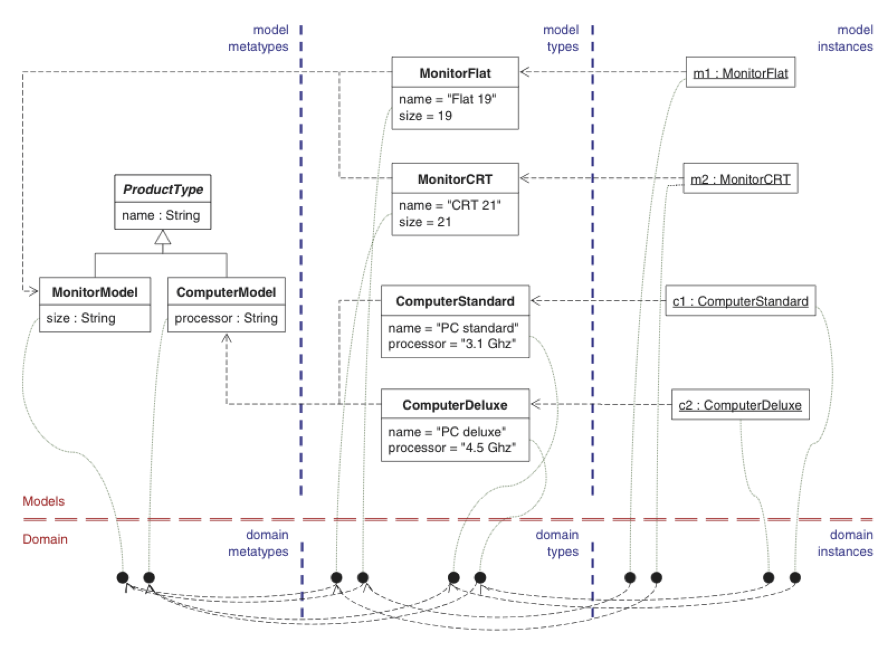
\includegraphics[width=0.9\textwidth]{images/chap3_model_clabject.png}
\caption{Example modeled using clabjects.}
\label{fig:model_clabject}
\end{figure} \\
Clabjects support any number of model classification levels, which creates a \textit{direct mapping} between ontological domain levels and modeling levels. This concept is visualized in figure ~\ref{fig:mapping_clabject}. This direct mapping requires that the solution structure reflects the problem structure as closely as possible. Now that we have introduced clabjects, a uniform way to support multiple domain levels, we can address the issue when elements in one level need to influence elements beyond its neighboring levels.

\begin{figure}[h!]
\centering
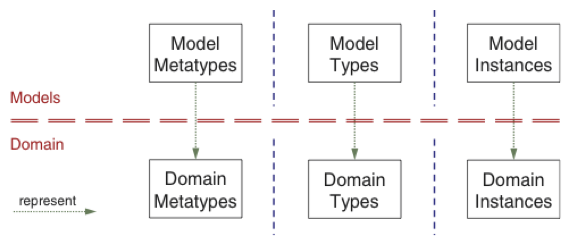
\includegraphics[width=0.9\textwidth]{images/chap3_mapping_direct.png}
\caption{Direct mapping between ontological domain levels and modeling levels.}
\label{fig:mapping_clabject}
\end{figure}

\subsection{Powertypes}

Using clabjects, the accidental complexity in the domain model was reduced significantly. However, there is one additional issue that needs to be addressed to allow multiple classification levels to be modeled naturally. This is the issue of \textit{deep characterization}. Deep characterization means that a type can influence the attributes of the types of its instances, as well as their object facets. Figure ~\ref{fig:deep_powertypes} shows an example of how Powertypes can be used to represent deep characterization. In this figure, we see two Powertypes, \texttt{ComputerModel} and \texttt{MonitorModel}. They respectively have slots \texttt{processor} and \texttt{size}. \\ \\
Let's have a look at the class \texttt{Computer}. This class has a \textit{power type} relationship with its Powertype \texttt{ComputerModel}. In general, if a superclass (e.g. \texttt{Computer}) is said to have a powertype (\texttt{ComputerModel}), then an instance of the Powertype (\texttt{ComputerStandard}) is only well-formed when it inherits from the superclass (\texttt{Computer}). Every derived class of a class inheriting from a Powertype should also be an instance of that Powertype (e.g. \texttt{ComputerDeluxe} inherits from \texttt{Computer} and is also an instance of the Powertype \texttt{ComputerModel}). Because the Powertypes contain slots (\texttt{processor} or \texttt{size}), we should instantiate those slots in a subclass (e.g. \texttt{ComputerStandard}). The slot \texttt{price} is only instantiated at the model instances level. \\ \\
Powertypes therefore control the type facet of powertype instances by means of inheritance. The powertype mechanism supports deep characterization, but as can be seen in the example only at the cost of introducing supertypes whose only purpose might be to provide a type facet for their subclasses. In the next section, we will solve this accidental complexity by introducing \textit{deep instantiation}.
\begin{figure}[h!]
\centering
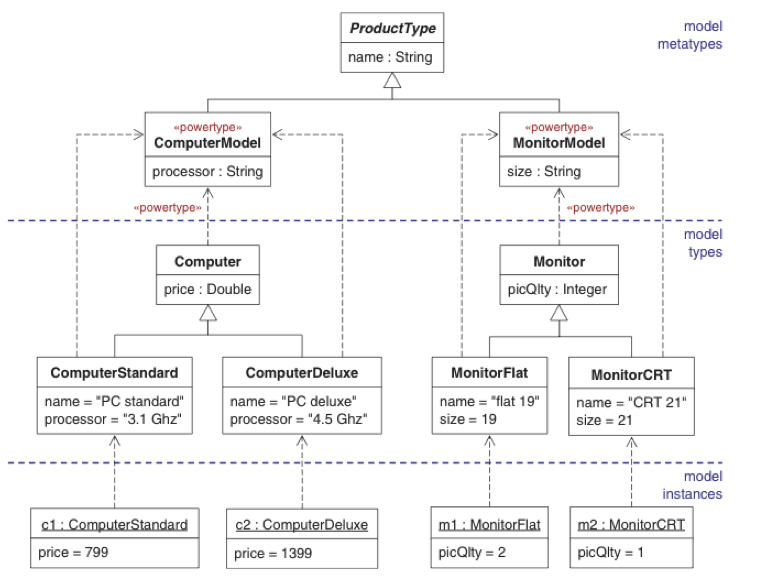
\includegraphics[width=0.9\textwidth]{images/chap3_deep_powertypes.png}
\caption{Deep characterization with powertypes.}
\label{fig:deep_powertypes}
\end{figure}

\subsection{Deep Instantiation}

Deep characterization is needed when a type should influence an entity beyond its immediate instances. In order to support deep characterization, we need a mechanism that backs it up in a concise way and minimizes accidental complexity introduced by deep characterization with powertypes. This mechanism is referred to as \textit{deep instantiation}.

\subsubsection{Potency}

Deep instantiation covers two concepts. One is the unification of attributes and slots into a single concept, which we refer to as \texttt{field}. The other concept extends clabjects and fields with an additional property known as \textit{potency}. Potency defines how deep an instantiation chain produced by a clabject or field may become. For example, when we create a field of potency two, it can produce an instantiation depth of two. Each instantiation of the field lowers the potency value by one, until the potency value equals zero. Entities with potency zero cannot be further instantiated and act like regular objects or slots. Figure ~\ref{fig:deep_potency} shows our domain model represented by deep characterization.
\begin{figure}[h!]
\centering
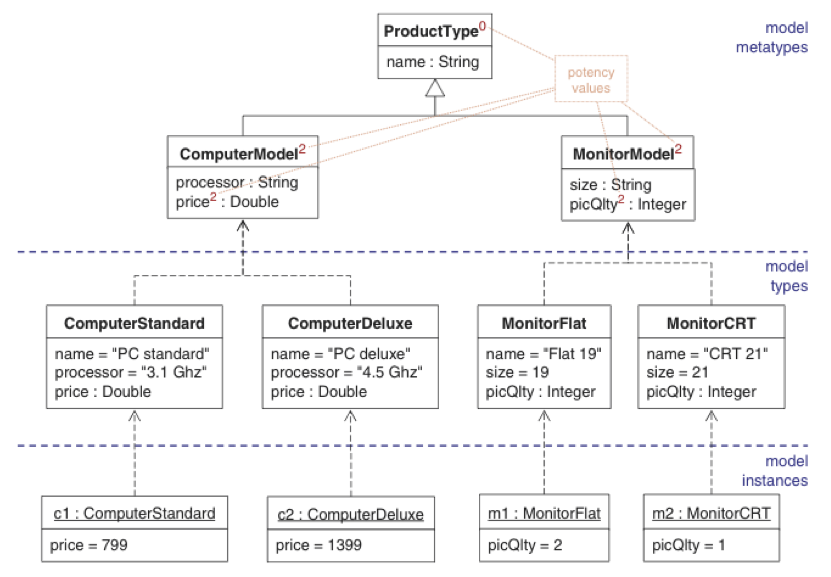
\includegraphics[width=0.9\textwidth]{images/chap3_deep_potency.png}
\caption{Deep characterization with potency.}
\label{fig:deep_potency}
\end{figure} \\
Every clabject has a maximum instantiation depth associated with it. This instantiation depth is indicated by the superscript next to the name of the clabject. For example, the clabject \texttt{ComputerModel} has an instantiation depth of two, but also has a field \texttt{price} of potency two at the model metatypes level. This is indicated by the superscript \textit{2} at the name of the field. After instantiating the clabject once, the potency of field \texttt{price} is reduced by one. Note that �price� acts like an attribute on this level (not visually indicated, but fields or clabjects without an explicit potency have a default value of 1). When we instantiate this clabject to an object \texttt{c1}, field \texttt{price} has turned into a slot that has a real value. Note that a potency value of zero for clabjects with non-zero potency fields allow us to create an \textit{abstract} (meta-)class. \\ \\
The example using potency introduces the least accidental complexity yet. It only allows computer and monitor types for computer and monitor instances respectively, without enhancing it with extra constraints. Furthermore, it doesn't require an extra superclass for merely providing a type facet like with Powertypes.

\section{Metadepth}

MetaDepth is a meta-modeling framework written in Java that uses a deep meta-modeling approach to support multiple programming levels. It introduces the concept of potency in meta-models and allows a developer to work in two ontological (domain) instantiation modes: \textit{strict} and \textit{extensible}, as shown in figure ~\ref{fig:metadepth_schemes}.
\begin{figure}[h!]
\centering
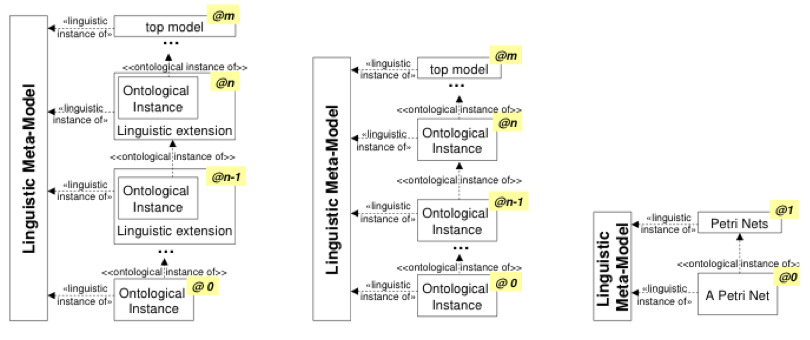
\includegraphics[width=0.9\textwidth]{images/chap3_metadepth_schemes.png}
\caption{MetaDepth instantiation schemes: extensible ontological instantiation (left) and strict ontological instantiation (center). Example of strict instantiation (right).}
\label{fig:metadepth_schemes}
\end{figure} \\
In the extensible case, it is possible to linguistically extend each ontological instance model (as depicted in the figure, on the left side). This means that instances of elements marked as \texttt{ext} can be extended with new linguistic attributes. We can also mark a complete model as extensible, allowing us to add new types and extend its elements. \\ \\
The alternative \textit{strict} case is similar to most meta-modeling environments in the sense that the top-level meta-model hardcodes all language concepts and can be subsequently instantiated ontologically. Note that such instances cannot be extended linguistically. This situation is depicted in the center of figure ~\ref{fig:metadepth_schemes}. For example, we could use this mode to describe the MOF meta-model at the highest level (and give it a potency of 2). This model could then be instantiated ontologically to describe meta-models for languages at potency 1. In turn, we can create instantiations (models) at potency level 0. Thus, the strict mode is similar to most meta-modeling environments, without restrictions on the number of meta-levels (i.e. deep meta-modeling). We will be using this \textit{strict} case in the collaborative modeling framework. \\ \\
On the right of figure ~\ref{fig:metadepth_schemes}, we see an example of the strict instantiation. Here we use the linguistic meta-model (see next section) to create a Petri Nets meta-model. The user then creates an ontological instance (i.e. a model) of the Petri Nets meta-model on the same linguistic meta-level.

\subsection{The Linguistic Meta-Model}

MetaDepth uses its own linguistic meta-model, inspired by MOF \cite{MetaDepth}. The framework is modified to accommodate an arbitrary number of meta-levels, using the concepts of deep instantiation and potency. Part of the linguistic meta-model is shown in figure ~\ref{fig:metadepth_ling}.
\begin{figure}[h!]
\centering
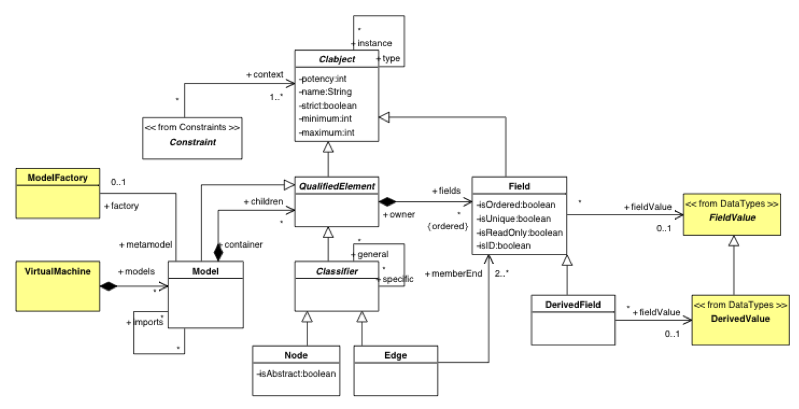
\includegraphics[width=0.9\textwidth]{images/chap3_metadepth_mm.png}
\caption{MetaDepth�s linguistic meta-model.}
\label{fig:metadepth_ling}
\end{figure} \\
The root class \texttt{Clabject} takes responsibility of handling the dual type/object facet of elements \cite{MetaDepth}. Therefore, it contains a potency attribute and links to its instances and types. \texttt{Constraints} can be attached to clabjects, as shown in the class diagram. All working models are managed by a \texttt{VirtualMachine} container, which is a \textit{singleton} object. \\
An example of the dual classification using a clabject and the two instance-of relationships is shown in figure ~\ref{fig:dual_class}. The ontological model stack depicts the user-defined (meta-)models, instantiated through the linguistic meta-model shown above. Notice that both fields \texttt{VAT} and \texttt{price} respectively have a potency of one and two in the \texttt{ProductType} meta-model. When instantiated one level lower, we fill in the \texttt{VAT} field, because we lowered its potency by one, which made it zero. The \texttt{price} field will subsequently be instantiated at the instance level.
\begin{figure}[h!]
\centering
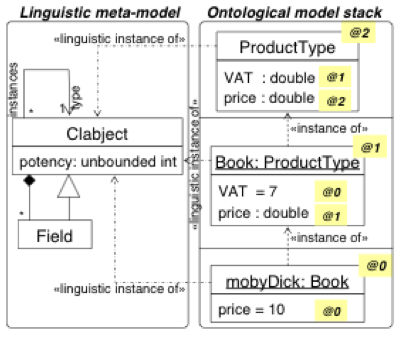
\includegraphics[width=0.4\textwidth]{images/chap3_dual_class.png}
\caption{Dual classification example.}
\label{fig:dual_class}
\end{figure}

\subsection{Tool Support}

MetaDepth models can be built through a Java API or through a \texttt{CommandShell} and a textual syntax, built with ANTLR \cite{ANTLR}. The storage of models is also done in this format. As an example, figure ~\ref{fig:model_ex} shows the three model dual classification example of figure ~\ref{fig:dual_class} in the textual notation. In this example, the model Store (with potency two) is extended linguistically through the Node \texttt{ProductType}. The \texttt{VAT} attribute in node \texttt{ProductType} has a potency of one (and a default value of 7.5), which means that it will be instantiated in its lower neighboring level. The \texttt{price} attribute has a potency of two. This is not visually indicated, but attributes are automatically assigned the parent (that of Model \texttt{Store}) potency if no explicit value is given. The majority of the collaborative modeling framework will be written in this textual syntax.
\begin{figure}[h!]
\centering
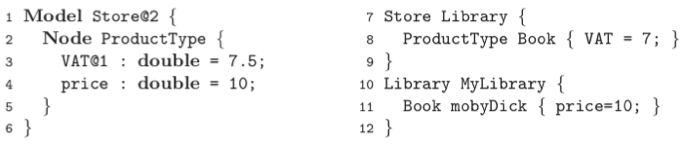
\includegraphics[width=0.9\textwidth]{images/chap3_model_ex.png}
\caption{Three model example.}
\label{fig:model_ex}
\end{figure} \\ \\
The Metadepth framework is integrated with Epsilon, a family of languages built on top of the Epsilon Object Language (EOL) \cite{EclipseEOL}, by communicating with the models through a connectivity layer. EOL can work with EMF models \cite{EclipseEMF}, but also with any other model technology that implements the interface of this connectivity layer. Metadepth works through this kind of interface and adds support to make EOL aware of multiple ontological levels. Using this approach, we can use EOL programs to create models, as shown in figure ~\ref{fig:eol}. We could also use EOL to define the semantics of a model (e.g. write a Petri Net simulator based on a model using the Epsilon Transformation Language (ETL) \cite{EclipseETL}).
\begin{figure}[h!]
\centering
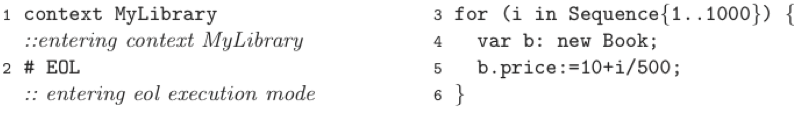
\includegraphics[width=0.9\textwidth]{images/chap3_eol.png}
\caption{An EOL program that populates a MetaDepth model.}
\label{fig:eol}
\end{figure}

\subsection{Constraints and Derived Attributes}

Constraints and actions in Metadepth are usually defined using Java or EOL. Just like clabjects and model fields, they have an assigned potency that indicates at which meta-level they have to be evaluated. Figure ~\ref{fig:metadepth_constraints} extends our Store example.
\begin{figure}[h!]
\centering
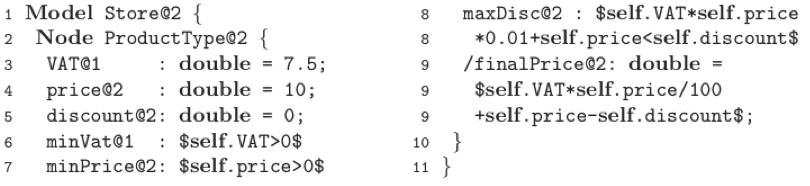
\includegraphics[width=0.9\textwidth]{images/chap3_metadepth_constraints.png}
\caption{Constraints and derived fields in Metadepth.}
\label{fig:metadepth_constraints}
\end{figure} \\
We have declared three constraints, on line 6, 7 and 8. An example of a derived field is given on line 9. The constraints are specified between two "\$" symbols and can be defined at the level of a clabject (as done in our example) or outside of it. The \texttt{minVat} constraint was given a potency of one, which means that it will be evaluated on the meta-level directly below. This constraint cannot access the value of fields with bigger potency, like \texttt{price}, as they may not have a value yet. The declaration of the derived field \texttt{finalPrice} is similar to a normal field, except that it is preceded by a backslash and may include fields with a lower potency.

\subsection{Controlling linguistic extensions}

A linguistic extension is interesting to permit unforeseen extensions to Domain Specific Languages spawning more than one level \cite{GenericMetaDepth}. In these languages, the top-most meta-model is usually highly generic, and linguistic extensions in lower levels could therefore be useful. Figure ~\ref{fig:ling_ext} shows an extension of our running example.
\begin{figure}[h!]
\centering
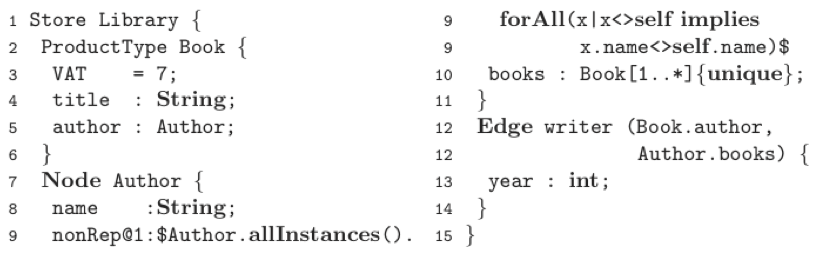
\includegraphics[width=0.9\textwidth]{images/chap3_ling_ext.png}
\caption{Linguistic extensions and associations in Metadepth.}
\label{fig:ling_ext}
\end{figure} \\
In the scenario above, we are interested in associating an author with \texttt{ProductType} instances. To achieve this, we linguistically extend the \texttt{Store} model by adding a new Node \texttt{Author}, which is an instance of \texttt{Node} in the linguistic meta-model (briefly discussed earlier). Authors are related to one or more books, modelled through the field books. The \texttt{\{unique\}} modifier ensures that a given \texttt{Author} is not related to the same \texttt{Book} twice.
\\ \\
In figure ~\ref{fig:ling_ext}, we also notice an association \texttt{writer}, that associates an author with a book. In Metadepth, associations can be annotated with fields by explicitly defining an \texttt{Edge} between their association ends. So in our example above, the association \texttt{writer} is instantiated as an \texttt{Edge} that relates books and authors. This \texttt{Edge} has got an extra field \texttt{year} that includes the year in which the book was written by that author.
%We could also define a more generic type of association. We could refer to linguistic types, like \texttt{Node}, when defining association ends. This makes sense if we want to specify that a certain association end is to be taken by any (linguistic) instance of \texttt{Node}.

\section{Other deep meta-modeling solutions}

Metadepth offers one solution to the problem of deep meta-modeling. However, other solutions exist, but not all are offered as integrated solutions. For example, DeepJava \cite{LiberateProgramming} is an extension of Java with the concept of potency, thus it cannot be considered as a framework. It does provide methods with potency, but needs special keywords to navigate up the type hierarchy in order to find attribute values. The constraints and computations for derived attributes in Metadepth can access type fields in a uniform way. This approach is preferred because it has the advantage that the number of meta-levels do not matter for a given field.
\\ \\
Next to DeepJava, another proposal for deep meta-modeling has been developed \cite{MultiLevelLangEng}. This tool is largely based on \textit{Ecore}. It considers multi-level constraints and proposes extending OCL to cope with multiple ontological meta-levels. This approach is similar to MetaDepth, but MetaDepth has got the ability of assigning \textit{potency} to constraints, which makes them easier to define on multiple meta-levels. More information about these concepts can be found in \cite{MultiLevelLangEng} and \cite{MetaDepth}.
